\documentclass[10pt,twocolumn]{article}
\usepackage[letterpaper,margin=0.7in,columnsep=0.25in]{geometry}
\usepackage{graphicx,booktabs,tabularx,array,hyperref,xcolor}
\usepackage[T1]{fontenc}
\definecolor{accent}{HTML}{058C9A}
\hypersetup{colorlinks=true,linkcolor=accent,urlcolor=accent,citecolor=accent}
\setlength{\parindent}{1em}
\setlength{\parskip}{0.2em}
\title{\textbf{DriftSentinel: Predictive Early Warning System for Concept Drift in Data Streams}}
\author{Laksh Raj\\Registration No. 23BDS0109\\Additional team members: \rule{3.2cm}{0.4pt}, \rule{3.2cm}{0.4pt}}
\date{Second Review Draft --- September 2026}

\begin{document}
\maketitle

\begin{abstract}
Concept drift changes the relationship between streaming inputs and outcomes, causing deployed models to lose accuracy. Conventional detectors such as ADWIN, DDM, and KSWIN react after statistical evidence accumulates; DriftSentinel instead asks whether drift will begin within the next five batches. The system converts online-classifier behaviour, rolling statistics, PSI, and confidence signals into sequences for Logistic Regression, GRU, LSTM, and Transformer models. Chronological, leakage-controlled experiments use deterministic SEA abrupt and gradual streams and the verified INSECTS abrupt-balanced stream; Elec2 is retained for streaming analysis but excluded from event scoring because authoritative onset labels are unavailable. Evaluation separates probabilistic PR-AUC from binary alarms and measures strict pre-onset coverage, lead time, false alarms, missed drift, causal recovery, and adaptation cost. GRU provides the strongest predictive warning coverage, but with high false alarms and reset cost. Reactive detectors are more conservative. The result is a reproducible prototype, dashboard, tests, and CI pipeline.
\end{abstract}

\noindent\textbf{Keywords:} concept drift, data streams, early warning, GRU, online learning, adaptation

\section{Introduction}
Streaming machine-learning systems operate under changing data distributions. A classifier that is adequate at deployment can degrade when the input distribution or the mapping between inputs and labels changes. Most operational drift detectors announce change after it becomes statistically visible. That is useful for diagnosis, but it may be too late to prepare retraining, route traffic, or increase human oversight.

DriftSentinel frames early warning as supervised sequence prediction. At batch $t$, the binary target equals one only when a verified drift onset lies in $(t,t+5]$. The matching evaluation window is $[\mathrm{onset}-5,\mathrm{onset})$, so an alert six batches before an onset receives no early-warning credit. This alignment prevents inflated lead time and coverage.

The main conclusion is deliberately qualified: GRU produced the best strict warning coverage among predictive models, but it also generated many false alarms and costly adaptations. Logistic Regression demonstrates that engineered rolling features contain useful signal. ADWIN and DDM remain conservative, with low false-alarm rates but limited pre-drift coverage.

\section{Literature Review}
Concept-drift work spans detection, adaptation, stream learning, and sequence modelling. Gama et al. provide the standard taxonomy and evaluation framing~\cite{gama2014}. DDM monitors online error statistics~\cite{gama2004}, whereas ADWIN uses adaptive windows to detect significant changes in a monitored mean~\cite{bifet2007}. KSWIN-style methods apply non-parametric window comparison; the project uses the River implementation as a binary reactive baseline, with KS-based stream comparison contextualized by Raab et al.~\cite{raab2020}. Souza et al. introduce INSECTS streams and discuss the difficulty of benchmarking with real-world data~\cite{souza2020}.

For sequence prediction, GRU~\cite{cho2014}, LSTM~\cite{hochreiter1997}, and Transformer attention~\cite{vaswani2017} offer different inductive biases. These architectures were not designed specifically for sparse, event-labelled drift forecasting, so they must be compared with a simple supervised baseline rather than assumed superior. River supplies the incremental-learning infrastructure used in the stream replay~\cite{montiel2021}.

\section{Research Gaps}
\begin{itemize}
\item Most drift detectors are reactive; strict prediction before onset is less emphasized.
\item Early-warning work rarely audits lead time, coverage, false alarms, missed drift, and adaptation cost together.
\item Deep sequence models need comparison with simple supervised baselines under identical chronological splits.
\item Verified, labelled real-world drift-event streams are limited, so provenance and event truth must be explicit.
\item Recovery claims require causal replay; a confidence proxy is not accuracy recovery after adaptation.
\end{itemize}

\section{Objectives}
The project builds a rolling-window feature pipeline, predicts drift within five batches, compares Logistic Regression, GRU, LSTM, and Transformer with ADWIN, DDM, and KSWIN, evaluates operational event metrics and recovery, and provides a reproducible pipeline with a Streamlit dashboard, tests, and CI.

\section{Proposed Methodology}
Figure~\ref{fig:method} summarizes the system. The raw stream is processed chronologically by an online classifier. Each batch yields rolling performance, PSI, confidence, and detector features. A sequence builder exposes historical windows to the predictive models. Thresholds are selected on validation data and frozen for test evaluation. Alerts can trigger a causal adaptation replay using only labels available at that time.

\begin{figure*}[t]
\centering
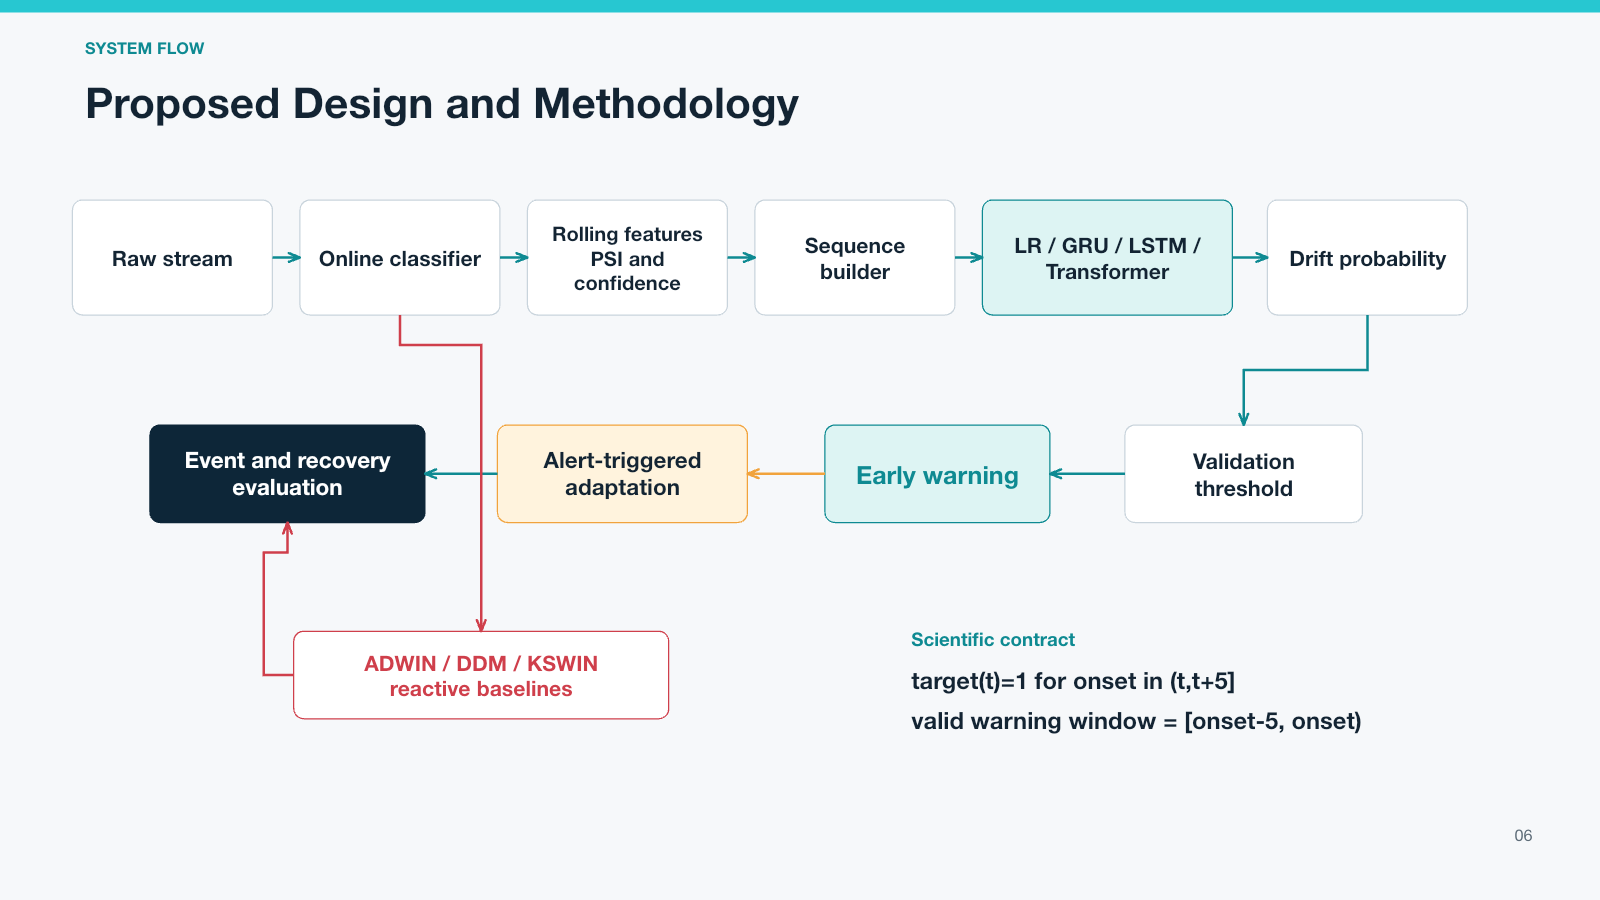
\includegraphics[width=0.94\textwidth]{assets/methodology_diagram.png}
\caption{DriftSentinel methodology and the five-batch target and warning contract. ADWIN, DDM, and KSWIN form the reactive comparison branch.}
\label{fig:method}
\end{figure*}

Event matching is one-to-one: one alert can match at most one onset, and one onset can receive credit from at most one eligible alert. Train, validation, and test are chronological. Scaling and threshold selection do not use test information.

\section{Dataset Description}
\begin{table*}[t]
\caption{Final benchmark datasets}
\centering\small
\begin{tabularx}{\textwidth}{@{}lcllX@{}}
\toprule
Dataset & Events & Use & Notes \\
\midrule
SEA abrupt & 10 & Event & Deterministic episodes \\
SEA gradual & 10 & Event & Deterministic episodes \\
INSECTS abrupt-balanced & 5 & Event & Verified mirror; hash documented \\
Elec2 & 0 verified & Analysis & No authoritative onset truth \\
\bottomrule
\end{tabularx}
\end{table*}

The original proposal listed Electricity, Airlines, Forest CoverType, and USENET. The Phase~1 repository actually contained Elec2, INSECTS abrupt-balanced, and SEA. The final benchmark uses streams available in the repository whose event truth could be verified or deterministically generated; it does not claim that all four proposal datasets were evaluated.

\begin{table*}[t]
\caption{Chronological class and event distribution}
\centering\small
\begin{tabular}{llrrrrr}
\toprule
Dataset & Split & Rows & Sequences & Positive & Negative & Events \\
\midrule
SEA abrupt & train & 356 & 347 & 30 & 317 & 6 \\
 & validation & 119 & 119 & 10 & 109 & 2 \\
 & test & 119 & 119 & 10 & 109 & 2 \\
SEA gradual & train & 356 & 347 & 30 & 317 & 6 \\
 & validation & 119 & 119 & 10 & 109 & 2 \\
 & test & 119 & 119 & 10 & 109 & 2 \\
INSECTS & train & 577 & 568 & 10 & 558 & 2 \\
 & validation & 158 & 158 & 5 & 153 & 1 \\
 & test & 315 & 315 & 10 & 305 & 2 \\
Elec2 & train & 495 & 486 & 0 & 486 & 0 \\
 & validation & 135 & 135 & 0 & 135 & 0 \\
 & test & 270 & 270 & 0 & 270 & 0 \\
\bottomrule
\end{tabular}
\label{tab:dist}
\end{table*}

A supervised event model is not presented as a meaningful trained predictor for Elec2 because the training split has zero positive targets. The event-scored benchmark therefore comprises SEA abrupt, SEA gradual, and INSECTS.

\section{Implementation Details}
Phase~1 produces auditable batches, rolling features, and reactive detector outputs. Phase~2 trains the four predictive models. Phase~3 performs strict event matching, threshold trade-off analysis, causal recovery replay, and reset-cost analysis. The dashboard exposes overview, drift timeline, model comparison, threshold trade-off, recovery and adaptation, and research-finding views.

The target and warning horizon are both five batches. Validation selects each predictive threshold; the selected checkpoint is restored before test inference. The adaptation replay warm-starts a reset classifier with at most 300 previously labelled rows. The reviewed repository has 43 passing tests and a passing CI workflow. Thus, the review requirement is accurately stated as: \emph{80\%+ implementation completed; full working prototype with dashboard, experiments, tests, and CI is ready.}

\section{Evaluation Metrics}
F1 evaluates batch-level target classification. PR-AUC is reported only for predictive methods that emit continuous probabilities. ADWIN, DDM, and KSWIN produce binary alarm flags here, so their PR-AUC is N/A rather than treated as directly comparable.

Warning lead time is the distance between a credited alert and onset within the strict five-batch window. Coverage is the fraction of events with a valid warning; missed drift is one minus coverage. Batch FAR is the fraction of negative target batches alarmed. Recovery batches count the time until rolling accuracy reaches 95\% of the pre-drift baseline. Recovery coverage records whether recovery occurs within the observation period. Adaptations per 100 batches quantify alert-triggered resets.

\section{Results and Analysis}
Table~\ref{tab:results} reports macro means across the three event-scored datasets. These are dataset-level means, not pooled event counts and not seed standard deviations; per-dataset seed variation is reported separately in the generated tables.

\begin{table*}[t]
\caption{Final macro comparison across event-scored datasets}
\centering\small
\begin{tabular}{lrrrrrrr}
\toprule
Method & F1 & PR-AUC & Lead & Coverage & FAR & Miss & Adapt/100 \\
\midrule
Logistic Regression & 0.1068 & 0.0909 & 0.00 & 0.0000 & 0.6652 & 1.0000 & 2.3592 \\
GRU & \textbf{0.1345} & \textbf{0.1039} & \textbf{1.83} & \textbf{0.3889} & 0.4972 & 0.6111 & 3.6415 \\
LSTM & 0.1222 & 0.0843 & 0.44 & 0.0556 & 0.7199 & 0.9444 & 1.6890 \\
Transformer & 0.0797 & 0.1020 & 0.11 & 0.0556 & 0.3086 & 0.9444 & 1.3425 \\
ADWIN & 0.0370 & N/A & 1.33 & 0.1667 & 0.0199 & 0.8333 & 1.9670 \\
DDM & 0.0513 & N/A & 0.67 & 0.1667 & 0.0083 & 0.8333 & 0.8777 \\
KSWIN & 0.0000 & N/A & 0.00 & 0.0000 & 0.0087 & 1.0000 & 0.8466 \\
\bottomrule
\end{tabular}
\label{tab:results}
\end{table*}

GRU achieved the strongest predictive warning coverage, 0.3889, with mean credited lead of 1.83 batches. This gain is not free: FAR was 0.4972 and its 3.6415 adaptations per 100 batches were the highest in the comparison. Logistic Regression did not cover a test event at the selected strict threshold, but F1 0.1068 and PR-AUC 0.0909 show that current rolling statistics contain useful supervised signal. ADWIN and DDM were more conservative: FAR 0.0199 and 0.0083 respectively, but coverage only 0.1667 each.

Pooled batch aggregation gives another view: Logistic Regression F1 is 0.1423 and GRU F1 is 0.1358. This does not contradict the macro result; it shows why pooled and per-dataset summaries must remain separate.

\subsection{Transformer Audit}
No bug was found in checkpoint restoration, masking, sequence dimensions, positional encoding, or logits and sigmoid usage. SEA training used 30 positive versus 317 negative targets, giving positive weight 10.57. INSECTS used 10 positive versus 558 negative targets, giving positive weight 55.8. The Transformer result is therefore documented as genuine underperformance under sparse supervision, not modified through outcome-driven tuning.

\begin{figure}[t]
\centering
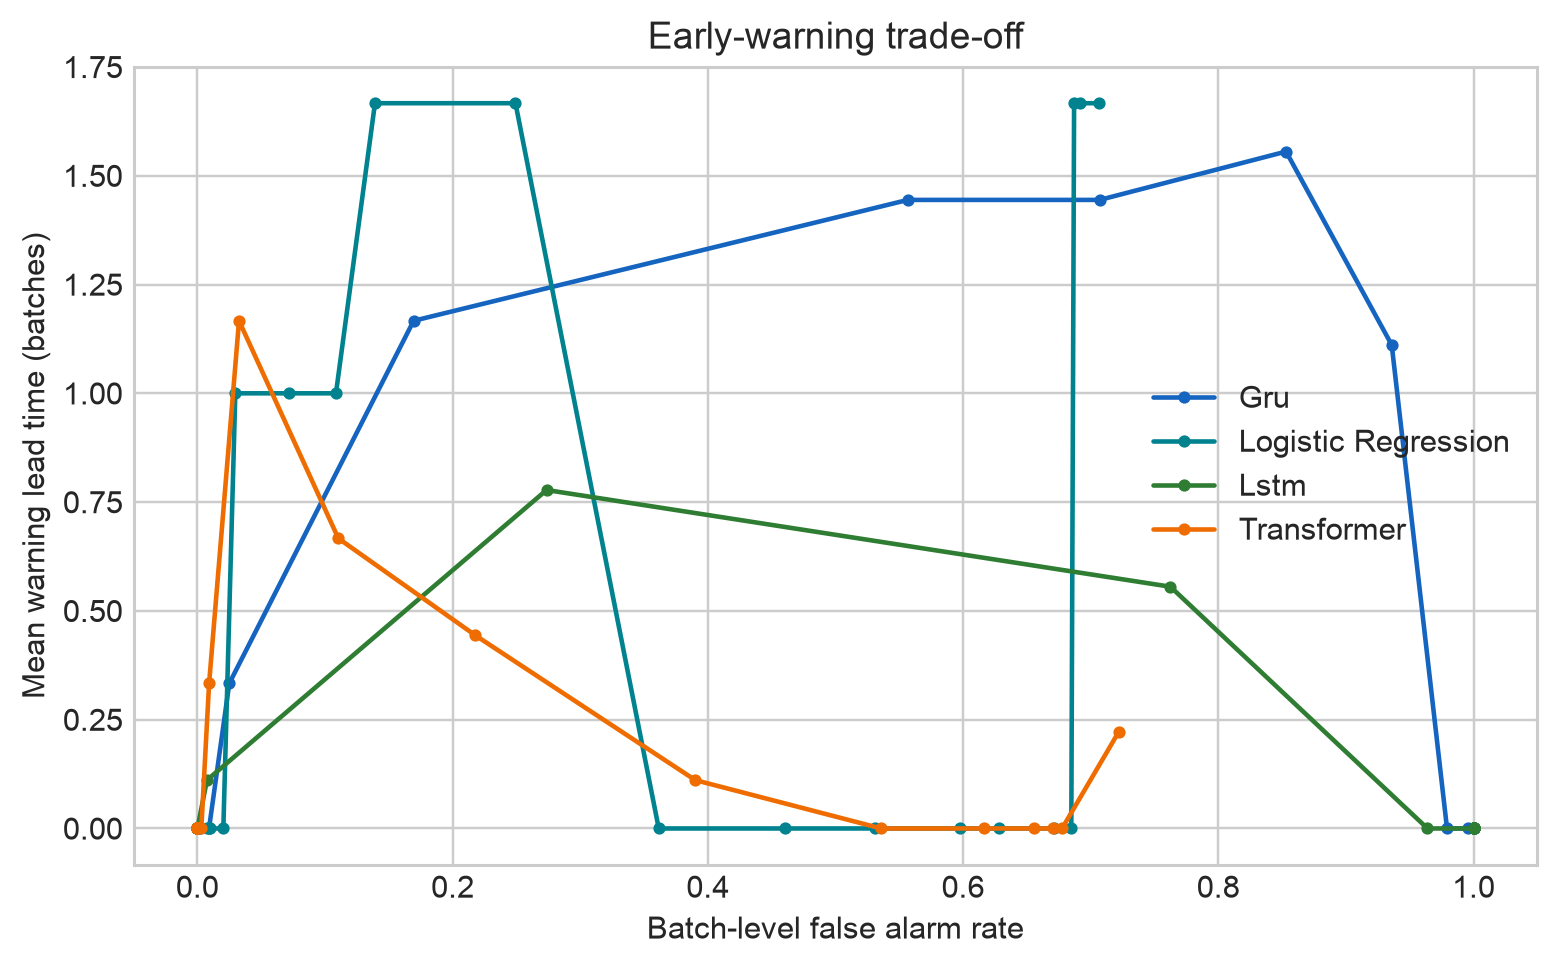
\includegraphics[width=\columnwidth]{../../results/figures/lead_time_vs_false_alarm.png}
\caption{Warning lead time and false-alarm trade-off.}
\label{fig:tradeoff}
\end{figure}

\begin{figure}[t]
\centering
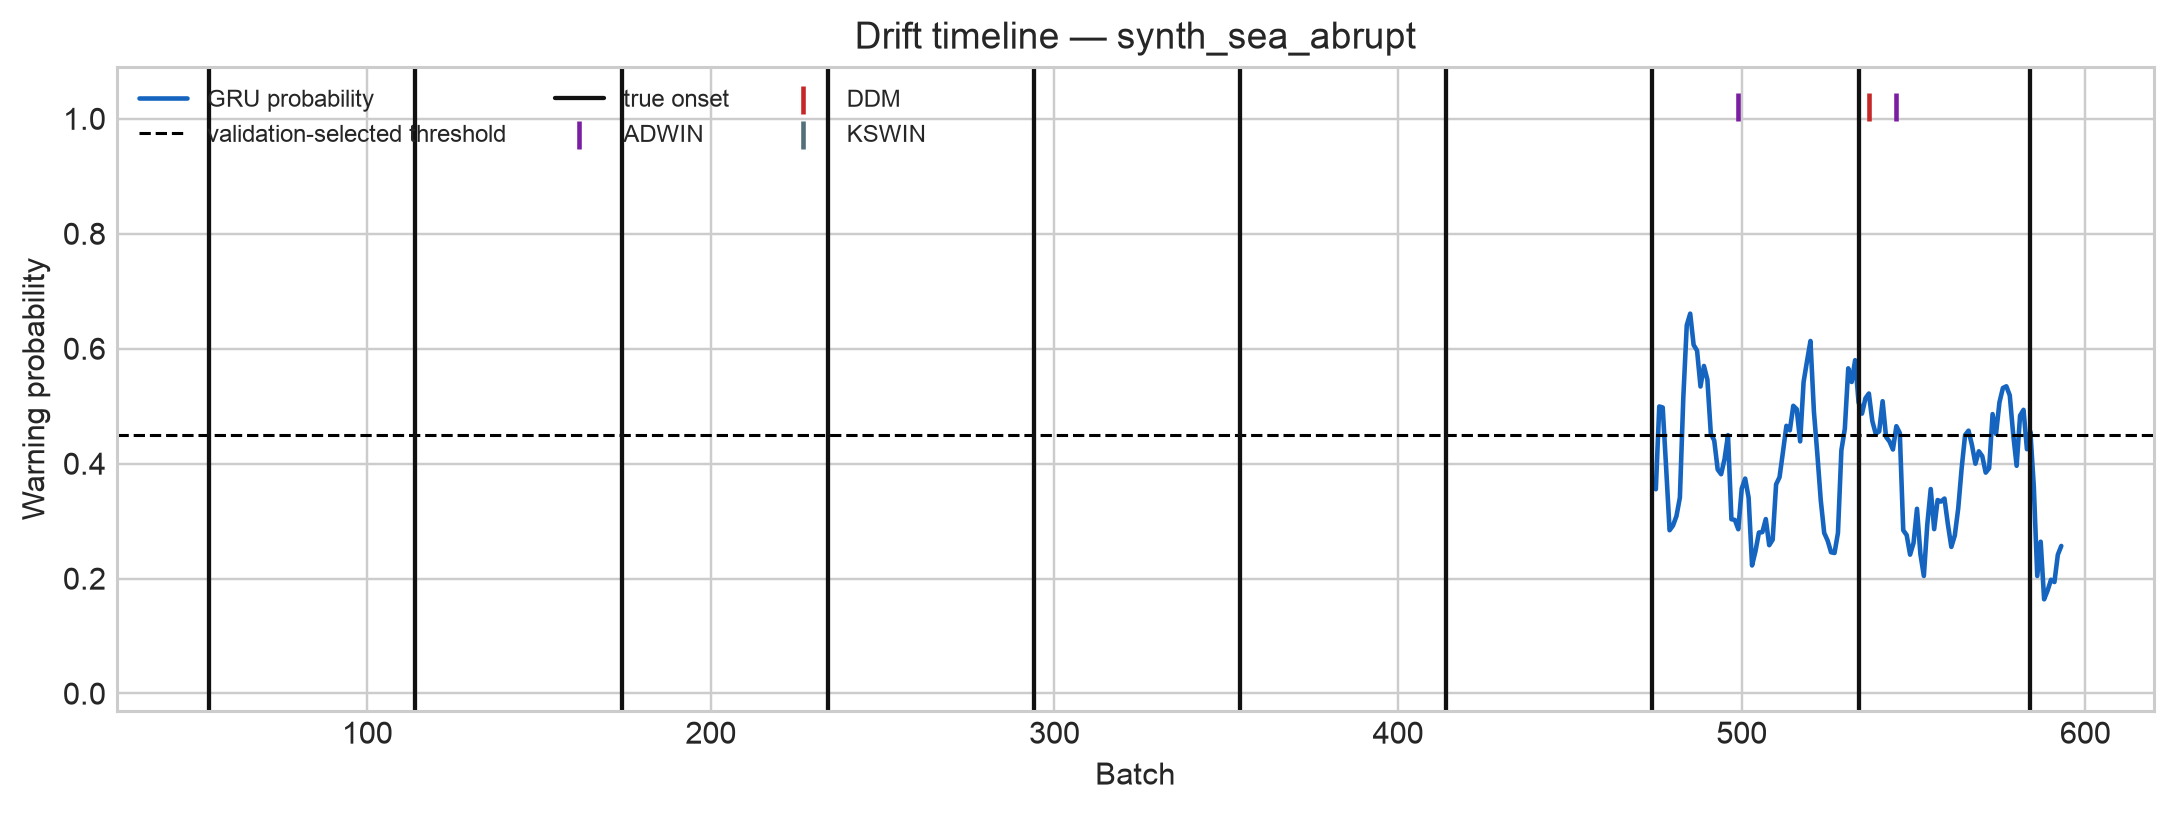
\includegraphics[width=\columnwidth]{../../results/figures/drift_timeline_synth_sea_abrupt.png}
\caption{Representative SEA abrupt timeline under strict five-batch warning eligibility.}
\label{fig:timeline}
\end{figure}

\begin{figure}[t]
\centering
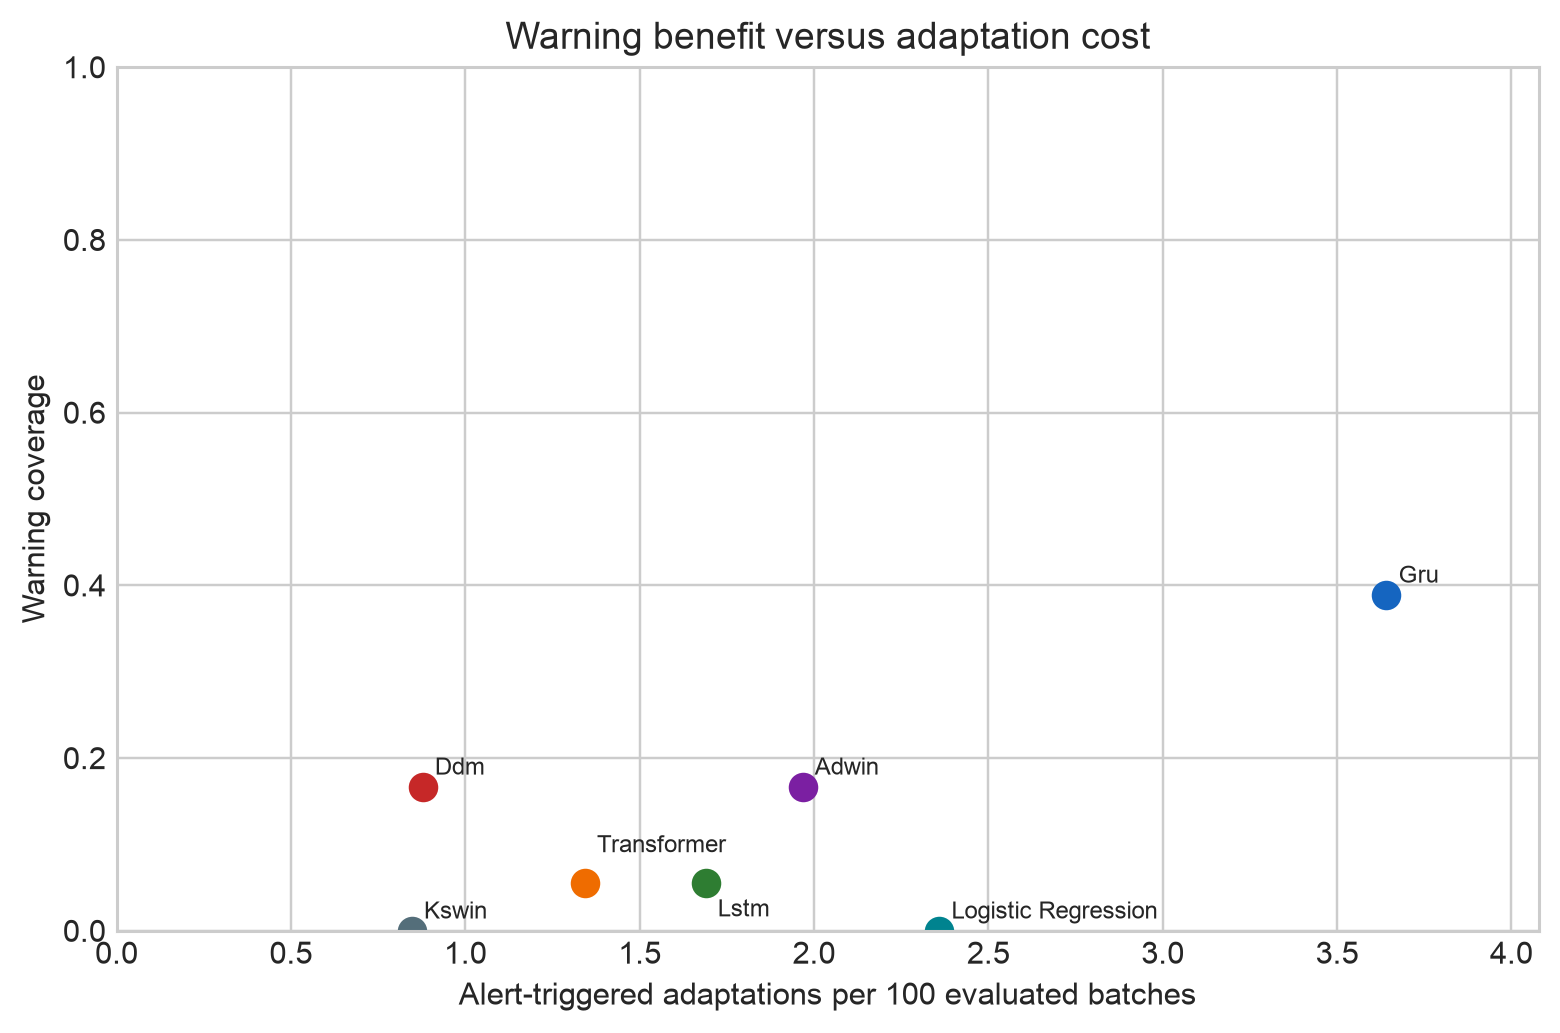
\includegraphics[width=\columnwidth]{../../results/figures/adaptation_cost_comparison.png}
\caption{Alert-triggered adaptation cost.}
\label{fig:adapt}
\end{figure}

\subsection{Recovery Replay}
Recovery is actual alert-triggered classifier adaptation, not a confidence proxy. Raw streams are replayed causally. At an alert, the classifier is reset and warm-started from at most 300 previously labelled observations; future rows are never used. Recovery is reached when rolling accuracy returns to 95\% of the pre-drift baseline. In the pooled reset audit, 60 of 67 GRU resets were false, for adaptation precision 0.1045. DDM was more conservative, with approximately 0.904 resets per 100 batches in the pooled view.

\section{Application}
Potential applications include financial fraud monitoring, industrial IoT sensor streams, demand forecasting, network intrusion detection, and recommendation systems. DriftSentinel is a research prototype and evaluation framework, not a production deployment or safety-critical decision system.

\section{Tangible Outcome Plan}
The selected tangible outcome is a conference paper on predictive concept-drift early warning. The planning target is the \href{https://icoicc.org.in/}{2027 4th International Conference on Intelligent and Cloud Computing (ICoICC 2027)}, an IEEE technically co-sponsored conference. This is a proposed target only: the work has not been submitted or accepted, and the call, indexing, eligibility, and faculty approval must be rechecked before communication.

The plan is to freeze evidence in September 2026, draft the 4--6 page manuscript in October, complete faculty review in November, revise and verify venue requirements in December, and submit by 31 January 2027 only if the venue remains suitable and approval is received. Any reviewer feedback will be addressed before communicating a revised or final version.

\section{Limitations}
The event benchmark contains three streams and 25 mapped events. Synthetic SEA episodes provide controlled truth but cannot represent every operational drift. Elec2 has no authoritative onsets and is excluded from event claims. False alarms and adaptation costs are high for the strongest warning model. Predictive PR-AUC and binary detector alarms answer different questions. Production latency, governance, and domain-specific economic costs have not yet been studied.

\section{Conclusion and Future Work}
DriftSentinel demonstrates that strict pre-onset prediction is feasible but difficult under sparse event supervision. GRU provides the strongest predictive event coverage, while ADWIN and DDM trade coverage for substantially lower FAR. Logistic Regression confirms that rolling statistics contain signal, and Transformer weakness reflects available supervision rather than an identified software defect. Future work should add verified event-labelled streams, calibrate alert utility against domain costs, explore self-supervised representations, and combine conservative reactive alarms with predictive probabilities.

\begin{thebibliography}{10}
\bibitem{gama2014} J. Gama, I. Zliobaite, A. Bifet, M. Pechenizkiy, and A. Bouchachia, ``A survey on concept drift adaptation,'' \emph{ACM Comput. Surv.}, vol. 46, no. 4, 2014, doi: 10.1145/2523813.
\bibitem{gama2004} J. Gama, P. Medas, G. Castillo, and P. Rodrigues, ``Learning with drift detection,'' in \emph{SBIA 2004}, pp. 286--295, doi: 10.1007/978-3-540-28645-5\_29.
\bibitem{bifet2007} A. Bifet and R. Gavaldà, ``Learning from time-changing data with adaptive windowing,'' in \emph{Proc. SIAM ICDM}, 2007, doi: 10.1137/1.9781611972771.42.
\bibitem{raab2020} C. Raab, M. Heusinger, and F.-M. Schleif, ``Reactive soft prototype computing for concept drift streams,'' \emph{Neurocomputing}, vol. 416, 2020, doi: 10.1016/j.neucom.2019.11.111.
\bibitem{souza2020} V. M. A. Souza et al., ``Challenges in benchmarking stream learning algorithms with real-world data,'' \emph{Data Min. Knowl. Discov.}, vol. 34, 2020, doi: 10.1007/s10618-020-00698-5.
\bibitem{cho2014} K. Cho et al., ``Learning phrase representations using RNN encoder--decoder for statistical machine translation,'' arXiv:1406.1078, 2014.
\bibitem{hochreiter1997} S. Hochreiter and J. Schmidhuber, ``Long short-term memory,'' \emph{Neural Comput.}, vol. 9, no. 8, 1997, doi: 10.1162/neco.1997.9.8.1735.
\bibitem{vaswani2017} A. Vaswani et al., ``Attention is all you need,'' in \emph{NeurIPS 30}, 2017.
\bibitem{montiel2021} J. Montiel et al., ``River: machine learning for streaming data in Python,'' \emph{J. Mach. Learn. Res.}, vol. 22, no. 110, 2021.
\bibitem{gama2010} J. Gama, \emph{Knowledge Discovery from Data Streams}. CRC Press, 2010.
\end{thebibliography}

\end{document}
